\documentclass[a4paper]{article}
\usepackage[T1]{fontenc}
\usepackage[utf8]{inputenc}
\usepackage[spanish]{babel}
\usepackage{mathtools}
\usepackage{amsmath}
\usepackage{graphics}
\usepackage{multicol}
\usepackage{listings}
\usepackage{color}
\usepackage{amsfonts}

\newcommand{\HRule}{\rule{\linewidth}{0.5mm}}


\definecolor{mygreen}{rgb}{0,0.6,0}
\definecolor{mygray}{rgb}{0.5,0.5,0.5}
\definecolor{mymauve}{rgb}{0.58,0,0.82}

\lstset{ %
  backgroundcolor=\color{white},   % choose the background color; you must add \usepackage{color} or \usepackage{xcolor}
  basicstyle=\footnotesize,        % the size of the fonts that are used for the code
  breakatwhitespace=false,         % sets if automatic breaks should only happen at whitespace
  breaklines=true,                 % sets automatic line breaking
  captionpos=b,                    % sets the caption-position to bottom
  commentstyle=\color{mygreen},    % comment style
  deletekeywords={...},            % if you want to delete keywords from the given language
  escapeinside={\%*}{*)},          % if you want to add LaTeX within your code
  extendedchars=true,              % lets you use non-ASCII characters; for 8-bits encodings only, does not work with UTF-8
  frame=single,                    % adds a frame around the code
  keywordstyle=\color{blue},       % keyword style
  language=C,                 % the language of the code
  morekeywords={*,...},            % if you want to add more keywords to the set
  numbers=left,                    % where to put the line-numbers; possible values are (none, left, right)
  numbersep=5pt,                   % how far the line-numbers are from the code
  numberstyle=\tiny\color{mygray}, % the style that is used for the line-numbers
  rulecolor=\color{black},         % if not set, the frame-color may be changed on line-breaks within not-black text (e.g. comments (green here))
  showspaces=false,                % show spaces everywhere adding particular underscores; it overrides 'showstringspaces'
  showstringspaces=false,          % underline spaces within strings only
  showtabs=false,                  % show tabs within strings adding particular underscores
  stepnumber=1,                    % the step between two line-numbers. If it's 1, each line will be numbered
  stringstyle=\color{mymauve},     % string literal style
  tabsize=2,                       % sets default tabsize to 2 spaces
  title=\lstname                   % show the filename of files included with \lstinputlisting; also try caption instead of title
}

\begin{document}

% Título
%	\begin{titlepage}
		\begin{center}

			\HRule \\[0.4cm]
			{ \huge \bfseries Paralelización del algoritmo de ordenamiento radixsort}
      \vspace{0.2cm}
      { \huge \bfseries usando MPI y OpenMP}\\[0.4cm]
			\HRule \\[0cm]

			\vspace{1cm}
			\textsc{\Large Arquitectura e Enxeñaría de Computadores}\\[0.5cm]
			\textsc{\Large Curso 2012/2013}\\[0.5cm]

		\end{center}


		\vspace{2cm}

		\begin{center}
		Penas Sabín, Darío \texttt{<dario.penas@udc.es>}\\
		\vspace{0.1cm}
		Pereira Guerra, Adrián \texttt{<adrian.pereira@udc.es>}\\
    https://github.com/adrisons/AEC
		\end{center}
		\vspace{1cm}

%	\end{titlepage}
% Índices

\tableofcontents
\vspace{3cm}
\clearpage

\section{Introducción}
  Radix sort es un algoritmo de ordenación cuyo rendimiento temporal en el peor caso es de $\mathcal{O}(kN)$ y de memoria $\mathcal{O}(k + N)$

Su principal característica es la utilización de un array de 10 posiciones denominado \emph{bucket}, inicializado en cada una de las iteraciones a 0 y que guarda en cada una de las posiciones del array el número de apariciones de cada una de las cifras coincidentes con la propia posición del \emph{bucket}.

Este \emph{bucket} es utilizado para calcular el propio \emph{bucket} acumulado con el que asignaremos una posición diferente a cada uno de los elementos en el array en \emph{b}.

En cada una de las iteraciones tenemos una variable llamada \emph{exp} que se irá multiplicando por 10 y que nos indica la cifra que miraremos en ese instante y que luego copiaremos a \emph{a}, que es el array inicial.

Este es el código de dicho algoritmo:

\begin{lstlisting}
// Uso del bucket en radix sort
while (m / exp > 0){
	int bucket[10] = {0};
	for (i = 0; i < n; i++){
		bucket[a[i] / exp % 10]++;
	}
	for (i = 1; i < 10; i++)
		bucket[i] += bucket[i - 1];
	for (i = n - 1; i >= 0; i--)
		b[--bucket[a[i] / exp % 10]] = a[i];
	for (i = 0; i < n; i++){
		a[i] = b[i];
	}
	exp *= 10;
}
\end{lstlisting}


\subsection{Ejemplo del algoritmo}

Vector inicial: 25 57 48 37 12 92 86 33\\

Los elementos quedarían ordenados de la siguiente manera:\\
0:\\
1:\\
2: 1\underline{2} 9\underline{2}\\
3: 3\underline{3}\\
4:\\
5: 2\underline{5}\\
6: 8\underline{6}\\
7: 5\underline{7} 3\underline{7}\\
8: 4\underline{8}\\
9:\\

El bucket, en vez de ser lo descrito anteriormente, quedaría con el número de elementos asignados a cada posición:\\
\\
0: 0\\
1: 0\\
2: 2\\
3: 1\\
4: 0\\
5: 1\\
6: 1\\
7: 2\\
8: 1\\
9: 0\\
\\

El vector después de esta iteración sería: 12 92 33 25 86 57 37 48\\

En la siguiente iteración nos centramos el la segunda cifra de cada uno de los elementos:\\
\\
0:\\
1: \underline{1}2\\
2: \underline{2}5\\
3: \underline{3}3 \underline{3}7\\
4: \underline{4}8\\
5: \underline{5}7\\
6: \\
7: \\
8: \underline{8}6\\
9: \underline{9}2\\

En esta ocasión el bucket quedaría de la siguiente forma:
\\
0: 0\\
1: 1\\
2: 1\\
3: 2\\
4: 1\\
5: 1\\
6: 0\\
7: 0\\
8: 1\\
9: 1\\

En este ejemplo el vector ya ha quedado ordenado: 12 25 33 37 48 57 86 92\\
	

\clearpage
\section{Paralelización con MPI}
	
Como este código es muy complicado de paralelizar, limitaremos el problema a dos procesadores, para simplificar el paso de datos.

Antes de comenzar a ordenar los datos es necesario calcular el máximo de todos los elementos, ya que influye en el número de ejecuciones del algoritmo, por lo tanto, es necesario que todos los procesos conozcan este dato. Todos los procesos tienen que ejecutar el mismo número de iteraciones, aunque puede que alguno no necesite hacer tantas, para sincronizar el paso de datos final, con el array ordenado.
Esto se hace con MPI\_Allreduce, que realiza la operación indicada (MPI\_MAX en este caso) sobre el dato indicado (m) y comparte el resultado con \textbf{todos} los procesos.
\begin{lstlisting}[frame=single]
	m = maximo(a, n);
	MPI_Allreduce(&m, &m, 1, MPI_INT, MPI_MAX, MPI_COMM_WORLD);
\end{lstlisting}

El bucket se recalcula en cada iteración, por lo que también es necesario compartirlo en cada iteración. Radixsort ordena en función de la suma acumulada del bucket.

El trabajo de realizar la suma acumulativa lo hace el proceso 1 y le manda el resultado al 0. Es necesario hacerlo de este modo, ya que se utiliza el bucket acumulado para calcular las posiciones destino de los elementos del array a, ordenándolo en cada iteración.

El cálculo de las posiciones destino se hace desde el final al principio del array a ordenar (así lo requiere el algoritmo). Además, se resta el bucket para obtener la posición destino por lo que, al paralelizarlo, es necesario secuencializar esta parte de los procesos, de modo que sigan el mismo orden que el secuencial. Para ello, los elementos se envían en orden \emph{inverso} de procesos (desde el proceso n al $n-1$, del $n-1$ al $n-2$, ...).

% a_intercambio
Es raro que, al dividir los datos a ordenar entre dos procesos, coincida que los datos del proceso 0 pertenezcan a la primera mitad del array a ordenar y los de proceso 1 a la segunda. Es decir, se va a tener que enviar algún dato de \texttt{P0} a \texttt{P1}. Para esto, se van almacenando los datos a intercambiar en un \emph{array de intercambio} y, al final de cada iteración, los procesos intercambian sus \texttt{a\_intercambio} y guardan los datos recibidos.

\begin{lstlisting}[frame=single]
// El P0 se queda esperando por los datos del P1
if(myrank==0){
	MPI_Recv(a_intercambio, elemTot, MPI_INT, 1, 3, MPI_COMM_WORLD, &status);
	MPI_Recv(&bucket[0], 10, MPI_INT, 1, 4, MPI_COMM_WORLD, &status);
	for(i=0;i<elemTot;i++){
		if(a_intercambio[i]!=-1){
			// Se adapta la posicion del otro proceso
			pos_envio = i % n;
			b[pos_envio] = a_intercambio[i];
		}
	}
	inicializar_array(&a_intercambio[0], elemTot, -1);
}
\end{lstlisting}

Este array tiene las dimensiones del array total. Se ha decidido implementarlo así, aunque pueda suponer una mayor carga de memoria, porque los procesos no siempre van a querer enviar datos en el mismo instante, lo que supondría que los procesos se quedaran esperando mútuamente y repercutiría mucho sobre el tiempo de ejecución.

\texttt{a\_intercambio} tiene las dimensiones del array total porque los elementos a intercambiar ya se guardan en la posición destino del otro proceso. De este modo, al guardar los datos en \texttt{a\_intercambio}, cada proceso tiene que adaptar la posición en la que se guarda al otro proceso.


Cuando el \texttt{P1} acaba una iteración, envía el bucket y el a\_intercambio al \texttt{P0} y se queda esperando por el a\_intercambio de \texttt{P0}.
\begin{lstlisting}[frame=single]
if(myrank==1){
	MPI_Send(a_intercambio, elemTot, MPI_INT, 0, 3, MPI_COMM_WORLD);
	MPI_Send(&bucket[0], 10, MPI_INT, 0, 4, MPI_COMM_WORLD);
	MPI_Recv(a_intercambio, elemTot, MPI_INT, 0, 5, MPI_COMM_WORLD, &status);

	for(i=0;i<n;i++){
		if(a_intercambio[i]!=-1){
			b[i] = a_intercambio[i];
		}
	}
	inicializar_array(&a_intercambio[0], elemTot, -1);
}
\end{lstlisting}

Al final de cada iteración del bucle, cada proceso recibe el \texttt{a\_intercambio} del otro proceso, lo guarda en su array \texttt{b} local y, finalmente, lo almacena en \texttt{a}.


Como se puede ver en la gráfica de la figura \ref{grafica_mpi}, no se consiguen mejoras en este ejemplo usando \texttt{MPI} con dos procesadores. Esto se debe al gran paso de datos entre procesadores, la secuencialización de un trozo del código y el hecho de sólo usar dos procesadores. Además, cuando mayor sea el máximo elemento del array a ordenar, más iteraciones tiene que hacer el algoritmo, mayor paso de datos en la paralelización \texttt{MPI} y mayor ineficiencia.

\begin{figure}[h]
	\centering
	\lstinputlisting{./res/tabla_mpi}
	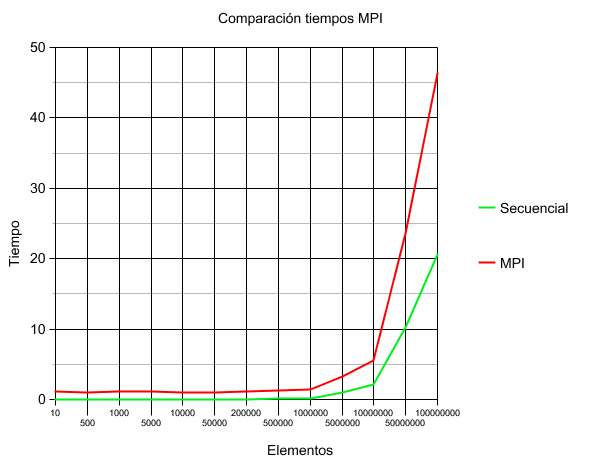
\includegraphics[width=1\textwidth]{./res/grafica_mpi}
	\label{grafica_mpi}
\end{figure}

\clearpage
\section{Paralelización con OpenMP}
	Como se comprueba en las pruebas, al emplear \texttt{MPI} sobre este problema no se obtiene ningún beneficio. Por ello, se aplicará \texttt{OpenMP} sobre el algoritmo secuencial en vez de hacerlo sobre el código paralelizado con \texttt{MPI}.

Como se había aclarado en el apartado de \texttt{MPI}, hay partes de nuestro programa que no son paralelizables (o con una complejidad demasiado elevada para el objetivo de este curso). A continuación se muestran partes del código sobre las que sí se puede aplicar \texttt{OpenMP}.

Al inicializar el array, por ejemplo, podemos dividir el trabajo entre varios threads.
\lstinputlisting[language=C]{./src/inicializacion_openmp.c}

Al hallar el máximo elemento del array también se nota mejoría al utilizar varios hilos.
\lstinputlisting[language=C]{./src/maximo_openmp.c}

Por último, al copiar los datos del array auxiliar \emph{b} en el array principal \emph{a} podemos usar varios hilos, ya que los datos no se pisan.
\lstinputlisting[language=C]{./src/copia_datos.c}


Aplicando estas pequeñas modificaciones se aprecia una gran mejora en el tiempo de ejecución con respecto al original (Figura \ref{Comparacion_tiempos} y Figura \ref{Comparacion_speedups}), y eso que la parte principal no se puede paralelizar (la que hace uso del bucket).

\begin{figure}[h!]
	\centering
	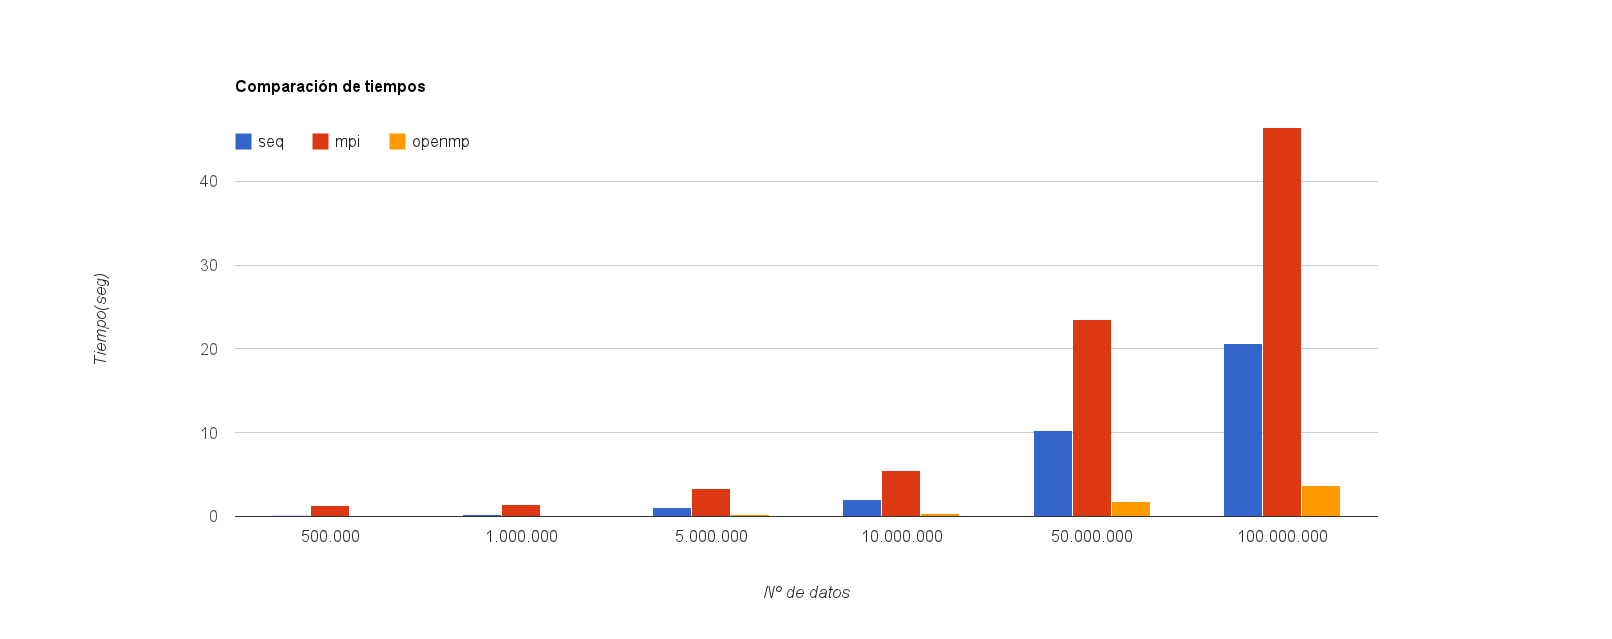
\includegraphics[width=1.3\textwidth]{./res/Comparacion_tiempos}
	\caption{Comparación tiempos}
	\label{Comparacion_tiempos}
\end{figure}

\begin{figure}[h!]
	\centering
	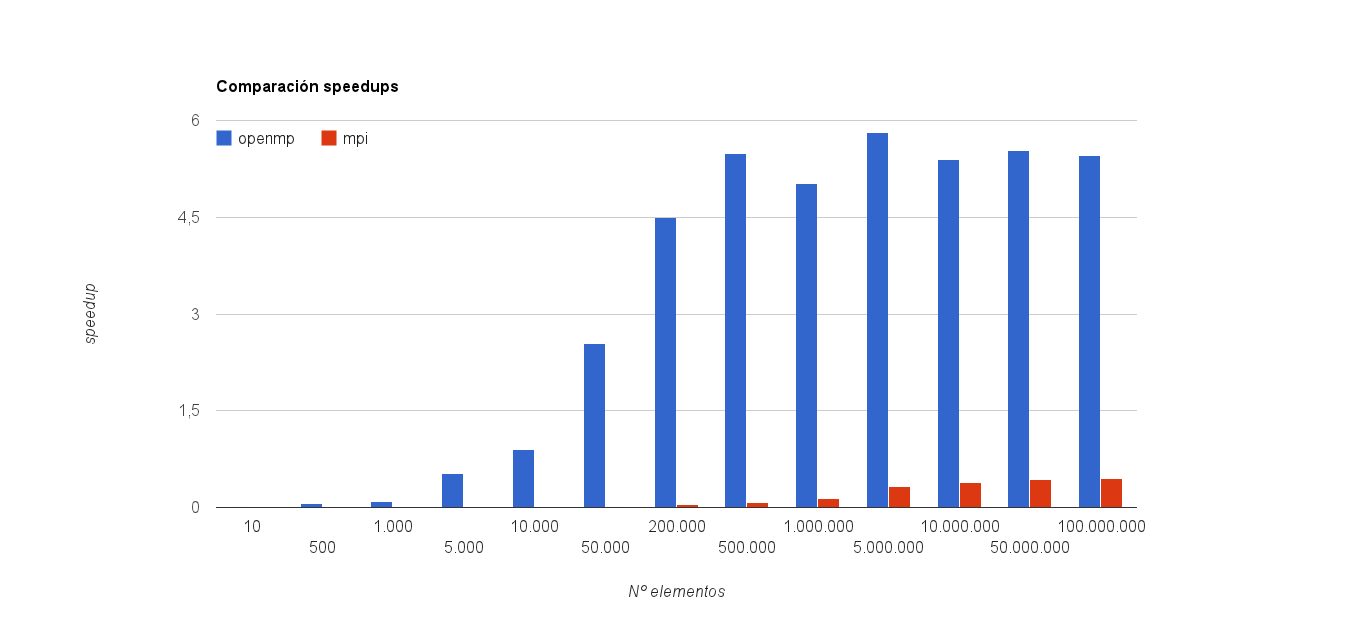
\includegraphics[width=1.3\textwidth]{./res/Comparacion_speedups}
	\caption{Comparación speedups}
	\label{Comparacion_speedups}
\end{figure}

\clearpage
\section{Conclusiones}
	Esta práctica nos ha resultado bastante complicada, ya que el problema era bastante complicado y no nos dimos cuenta de todas las restricciones en un principio. De todos modos, nos ha parecido muy interesante ver que se pueden mejorar mucho los tiempos de ejecución de ciertos programas, aunque pueda costar bastante esfuerzo.


Nuestra percepción general de la asignatura es positiva, debido sobre todo a la segunda parte que, en vez de ver el paralelismo desde un punto de vista teórico, experimentamos a trabajar realmente con él y aprendemos más, en nuestra opinión. Preferimos aprender las cosas de este modo que no viéndolo sólamente de manera teórica en clase.



\clearpage
\appendix

\section{Código secuencial}\label{secuencial.c}
\lstinputlisting[language=C]{./src/secuencial.c}

\section{main con MPI}\label{main.c}
\lstinputlisting[language=C]{./src/main.c}

\section{Implementación radixsort con MPI}\label{radixsort_mpi.c}
\lstinputlisting[language=C]{./src/radixsort_mpi.c}

\section{main con OpenMP}\label{main.c}
\lstinputlisting[language=C]{./src/main_openmp.c}

\section{Implementación radixsort con OpenMP}\label{radixsort_mpi.c}
\lstinputlisting[language=C]{./src/radixsort_openmp.c}
\end{document}
